% Options for packages loaded elsewhere
\PassOptionsToPackage{unicode}{hyperref}
\PassOptionsToPackage{hyphens}{url}
\PassOptionsToPackage{dvipsnames,svgnames,x11names}{xcolor}
%
\documentclass[
  11pt,
  a4paper,
]{article}
\usepackage{amsmath,amssymb}
\usepackage{iftex}
\ifPDFTeX
  \usepackage[T1]{fontenc}
  \usepackage[utf8]{inputenc}
  \usepackage{textcomp} % provide euro and other symbols
\else % if luatex or xetex
  \usepackage{unicode-math} % this also loads fontspec
  \defaultfontfeatures{Scale=MatchLowercase}
  \defaultfontfeatures[\rmfamily]{Ligatures=TeX,Scale=1}
\fi
\usepackage{lmodern}
\ifPDFTeX\else
  % xetex/luatex font selection
  \setmainfont[]{Liberation Serif}
\fi
% Use upquote if available, for straight quotes in verbatim environments
\IfFileExists{upquote.sty}{\usepackage{upquote}}{}
\IfFileExists{microtype.sty}{% use microtype if available
  \usepackage[]{microtype}
  \UseMicrotypeSet[protrusion]{basicmath} % disable protrusion for tt fonts
}{}
\makeatletter
\@ifundefined{KOMAClassName}{% if non-KOMA class
  \IfFileExists{parskip.sty}{%
    \usepackage{parskip}
  }{% else
    \setlength{\parindent}{0pt}
    \setlength{\parskip}{6pt plus 2pt minus 1pt}}
}{% if KOMA class
  \KOMAoptions{parskip=half}}
\makeatother
\usepackage{xcolor}
\usepackage[margin=21mm]{geometry}
\usepackage{longtable,booktabs,array}
\usepackage{calc} % for calculating minipage widths
% Correct order of tables after \paragraph or \subparagraph
\usepackage{etoolbox}
\makeatletter
\patchcmd\longtable{\par}{\if@noskipsec\mbox{}\fi\par}{}{}
\makeatother
% Allow footnotes in longtable head/foot
\IfFileExists{footnotehyper.sty}{\usepackage{footnotehyper}}{\usepackage{footnote}}
\makesavenoteenv{longtable}
\usepackage{graphicx}
\makeatletter
\def\maxwidth{\ifdim\Gin@nat@width>\linewidth\linewidth\else\Gin@nat@width\fi}
\def\maxheight{\ifdim\Gin@nat@height>\textheight\textheight\else\Gin@nat@height\fi}
\makeatother
% Scale images if necessary, so that they will not overflow the page
% margins by default, and it is still possible to overwrite the defaults
% using explicit options in \includegraphics[width, height, ...]{}
\setkeys{Gin}{width=\maxwidth,height=\maxheight,keepaspectratio}
% Set default figure placement to htbp
\makeatletter
\def\fps@figure{htbp}
\makeatother
\setlength{\emergencystretch}{3em} % prevent overfull lines
\providecommand{\tightlist}{%
  \setlength{\itemsep}{0pt}\setlength{\parskip}{0pt}}
\setcounter{secnumdepth}{-\maxdimen} % remove section numbering
\ifLuaTeX
\usepackage[bidi=basic]{babel}
\else
\usepackage[bidi=default]{babel}
\fi
\babelprovide[main,import]{japanese}
\ifPDFTeX
\else
\babelfont{rm}[]{Liberation Serif}
\fi
% get rid of language-specific shorthands (see #6817):
\let\LanguageShortHands\languageshorthands
\def\languageshorthands#1{}
\usepackage{xeCJK}
\setCJKmainfont{Noto Serif CJK JP}
\setCJKsansfont{Noto Sans CJK JP}
\usepackage{booktabs}
\usepackage{microtype}
\usepackage{fancyhdr}
\usepackage{needspace}
\usepackage{float}
\floatplacement{figure}{H}
\setCJKmonofont{Noto Sans CJK JP}
\pagestyle{fancy}
\fancyhf{}
\fancyhead[L]{\small Creative Self | Literature working notes}
\fancyfoot[R]{\small\thepage}
\setlength{\headheight}{15pt}
\setlength{\emergencystretch}{3em}
\setlength{\parskip}{0.55em}
\setlength{\parindent}{0pt}
\renewcommand{\arraystretch}{1.24}
\ifLuaTeX
  \usepackage{selnolig}  % disable illegal ligatures
\fi
\usepackage{bookmark}
\IfFileExists{xurl.sty}{\usepackage{xurl}}{} % add URL line breaks if available
\urlstyle{same}
\hypersetup{
  pdftitle={Creative Self の理論体系を理解する},
  pdflang={ja},
  colorlinks=true,
  linkcolor={blue},
  filecolor={Maroon},
  citecolor={Blue},
  urlcolor={blue},
  pdfcreator={LaTeX via pandoc}}

\title{Creative Self の理論体系を理解する}
\usepackage{etoolbox}
\makeatletter
\providecommand{\subtitle}[1]{% add subtitle to \maketitle
  \apptocmd{\@title}{\par {\large #1 \par}}{}{}
}
\makeatother
\subtitle{Jussupow et al.~(2026) と Karwowski et al.~(2019)
の比較・原著に基づく概念の再構成}
\author{}
\date{}

\begin{document}
\maketitle

\section{1.
この資料の目的と結論}\label{ux3053ux306eux8cc7ux6599ux306eux76eeux7684ux3068ux7d50ux8ad6}

本資料は研究計画のための学習・検討資料であり、提出原稿ではない。Jussupow
et al.~(2026) の Creative Self
を理解するには、創造性に関する自己信念を分類する Karwowski et al.~(2019)
の体系をそのまま当てはめるのではなく、自己の社会的構成、自己呈示、社会的承認、創造的主体性、作品と自己の関係を区別する必要がある。v3
の九原著に今回追加された六原著を加え、15点の提供資料の該当箇所を一次資料として参照する。出典IDと引用文は別冊
Evidence Ledger に対応する。

\textbf{結論：} Jussupow の Creative Self
は、創造的主体性を発揮して成果物を生み出す能力に根ざした自己の一部分である。それが表現された作品を通じて他者から承認されるという理論を構築する。実験ではその自己の強さ・変化を直接数値化するのではなく、行動、作品についての自己評価、所有感、観客の評価についての予想などを観察する。したがって「Creative
Self が低下した」ことと「Creative Self
の呈示が弱まった」ことを混同してはいけない。

\textbf{資料の根拠区分：} A＝提供原著から該当箇所を確認。B＝Jussupow
本文での引用用途と書誌を確認、引用先の全文は未確認。C＝別冊に記載の暫定的な尺度対応・要検証事項。資料中の図と応用例は説明用の再構成であり、原著の検証済み統計モデルや逐語的定義ではない。

\subsection{1.1 読書の地図}\label{ux8aadux66f8ux306eux5730ux56f3}

\begin{figure}
\centering
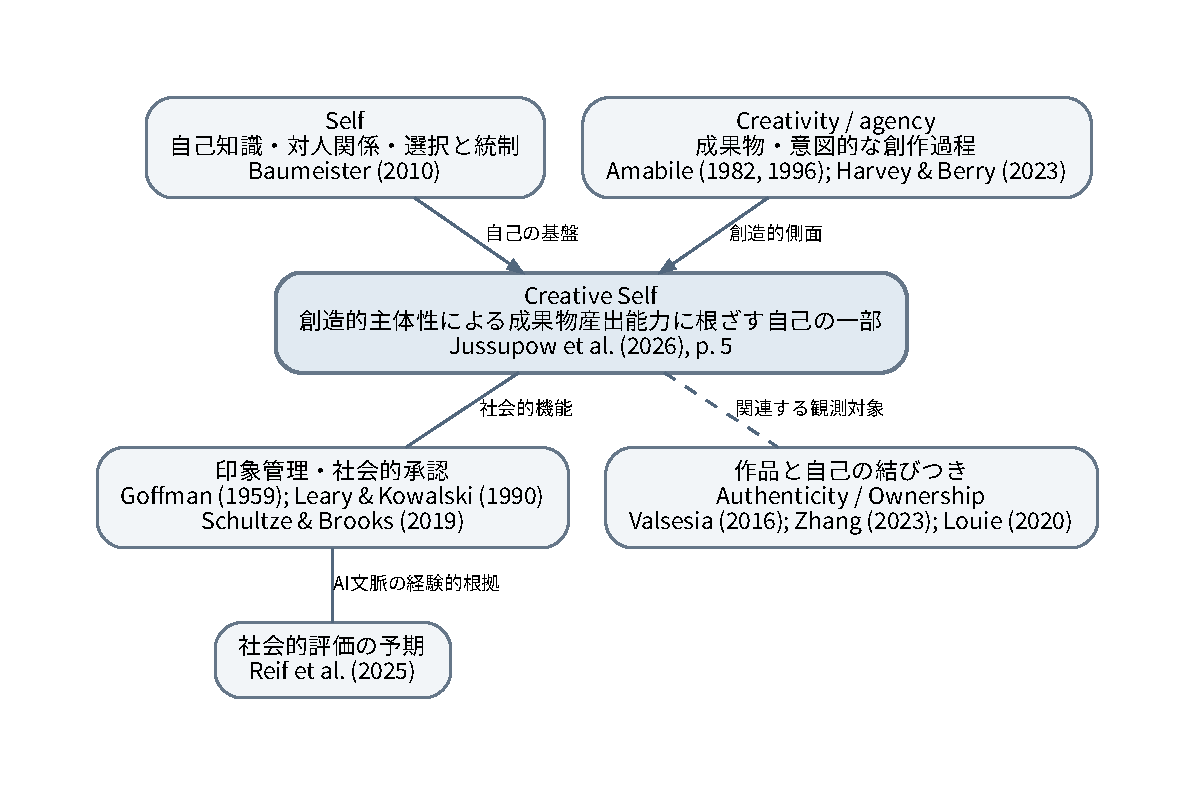
\includegraphics[width=0.95\textwidth,height=\textheight]{figures/theory.pdf}
\caption{図1　理論の構成要素と文献の役割（説明用概念図）。矢印は定義に寄与する関係、破線は関連する観測対象。因果の実証を表さない。}
\end{figure}

\section{2. 二つの Creative Self
のアプローチ}\label{ux4e8cux3064ux306e-creative-self-ux306eux30a2ux30d7ux30edux30fcux30c1}

\subsection{2.1 Karwowski：Creative Self-Beliefs
の体系}\label{karwowskicreative-self-beliefs-ux306eux4f53ux7cfb}

Karwowski, Lebuda \& Beghetto (2019), pp.~397--404 {[}K01--K05{]}
は、創造的自己を広いアイデンティティの一部とみなし、創造性についての自己信念を概念的に区別する。性格特性とも区別し、信念の時間志向、特定性、可変性に着目する。Table
19.1 は次の三分類を与える。

\begin{longtable}[]{@{}
  >{\raggedright\arraybackslash}p{(\columnwidth - 4\tabcolsep) * \real{0.3333}}
  >{\raggedright\arraybackslash}p{(\columnwidth - 4\tabcolsep) * \real{0.3333}}
  >{\raggedright\arraybackslash}p{(\columnwidth - 4\tabcolsep) * \real{0.3333}}@{}}
\toprule\noalign{}
\begin{minipage}[b]{\linewidth}\raggedright
上位分類
\end{minipage} & \begin{minipage}[b]{\linewidth}\raggedright
構成概念
\end{minipage} & \begin{minipage}[b]{\linewidth}\raggedright
典型的な問い（説明例）
\end{minipage} \\
\midrule\noalign{}
\endhead
\bottomrule\noalign{}
\endlastfoot
Creative Confidence & CSE & この条件で独創的な案を作れるか \\
Creative Confidence & CSC & 普段から独創的な案を考えるのが得意か \\
Creative Self-Awareness & Creative Metacognition &
何が得意で、いつどう創造的に行動するか \\
Creative Self-Awareness & Creative Mindset & 創造的能力は伸ばせるか \\
Creative Self-Image & Perceived Value of Creativity / Creative Personal
Identity に関連する信念 & 創造性は自己にとって重要か \\
\end{longtable}

CSE は課題・状況・達成水準を伴う将来の遂行可能性の判断、CSC
は比較的安定した全般的・回顧的な評価（pp.~398--401）。CMC
は強み・弱みと状況についての知識、また正確性・調整の問題を含む（pp.~401--402）。Mindset
は能力の固定性／可変性についての信念（pp.~402--403）。Self-Image
は創造的活動・能力・志向が自己にどう位置づくか（pp.~403--404）。これらは独立に変わりうる。

\subsection{2.2 Jussupow：Creative Self
の社会的呈示}\label{jussupowcreative-self-ux306eux793eux4f1aux7684ux5448ux793a}

Jussupow et al.~(2026), §2.4, p.~5 {[}J01--J05{]} は Self
を自分が何者かについての反省的理解として導入し、その中の創造的側面を定義する。創造的な成果物を通じて自己を他者に提示し、観客が人間の創造的主体性を承認するかどうかが、どのような創作行動を選択するかに影響すると理論化する。

\begin{longtable}[]{@{}
  >{\raggedright\arraybackslash}p{(\columnwidth - 4\tabcolsep) * \real{0.3333}}
  >{\raggedright\arraybackslash}p{(\columnwidth - 4\tabcolsep) * \real{0.3333}}
  >{\raggedright\arraybackslash}p{(\columnwidth - 4\tabcolsep) * \real{0.3333}}@{}}
\toprule\noalign{}
\begin{minipage}[b]{\linewidth}\raggedright
比較軸
\end{minipage} & \begin{minipage}[b]{\linewidth}\raggedright
Karwowski (2019)
\end{minipage} & \begin{minipage}[b]{\linewidth}\raggedright
Jussupow (2026)
\end{minipage} \\
\midrule\noalign{}
\endhead
\bottomrule\noalign{}
\endlastfoot
中核 & 自己に関する創造的信念 & 創造的主体性に根ざす自己と社会的承認 \\
理論の焦点 & 信念の区分・創造的行動 & 自己呈示・印象管理・撤退 \\
分析対象 & 人・課題・領域に関する信念 & 人、作品、観客、相互作用 \\
時間 & CSE は状況的、CSC 等は比較的安定 &
創作行動・作品との関係は状況的。自己自体の時間的安定性は特定していない \\
尺度 & CSE, CSC, CPI 等 & 行動ログ、真正性、所有感、観客反応の予期等 \\
共通点 & 自己と創造的行動の関係 & 自己と創造的行動の関係 \\
\end{longtable}

両者を完全に対立させる必要はない。Karwowski
も創造性を自己の一部として捉え、社会的・環境的影響を扱う。一方、Jussupow
は CSE や CPI の強度を独立尺度として測定していない。Creative Self-Image
/ CPI
は最も近い比較対象だが、自己における創造性の価値と作品を通じた他者からの承認は同じではない。

\textbf{SSCS の位置づけ：} SSCS (Karwowski et al., 2018) は trait-like
CSE と CPI を測る。Jussupow 最終版本文に SSCS、Karwowski、creative
self-efficacy の記載は確認されない（付録の統制変数は未確認）。Jussupow
の枠組みを単独採用するなら SSCS
は必須ではない。創造的アイデンティティの重要性を調整変数として検討する場合に限り、別構成概念として導入する余地がある。

\textbf{対照例：}
写真家が「自分は創造的な写真を撮れる」と確信しながら、展覧会で工夫を理解されないと予想して作品を簡略化する場合、CSE
は高くても呈示は弱くなる。反対に、技術に自信がなくても、創作が自己に重要で、他者に努力を認めてもらいたい人もいる。能力への信念、自己における重要性、承認の期待、実際の関与を分けて考える。

\section{3. Self の理論的基盤：Baumeister
(2010)}\label{self-ux306eux7406ux8ad6ux7684ux57faux76e4baumeister-2010}

\subsection{3.1
一つの性質ではなく三つの基盤}\label{ux4e00ux3064ux306eux6027ux8ceaux3067ux306fux306aux304fux4e09ux3064ux306eux57faux76e4}

Baumeister (2010), Chapter 5, p.~142（提供PDF p.~4）{[}B01--B03{]}
は、自己の研究を単一の根本現象に還元しようとしてうまくいかなかったと述べ、三つの基盤を提示する。

\begin{longtable}[]{@{}
  >{\raggedright\arraybackslash}p{(\columnwidth - 4\tabcolsep) * \real{0.3333}}
  >{\raggedright\arraybackslash}p{(\columnwidth - 4\tabcolsep) * \real{0.3333}}
  >{\raggedright\arraybackslash}p{(\columnwidth - 4\tabcolsep) * \real{0.3333}}@{}}
\toprule\noalign{}
\begin{minipage}[b]{\linewidth}\raggedright
基盤
\end{minipage} & \begin{minipage}[b]{\linewidth}\raggedright
意味
\end{minipage} & \begin{minipage}[b]{\linewidth}\raggedright
創造活動の例
\end{minipage} \\
\midrule\noalign{}
\endhead
\bottomrule\noalign{}
\endlastfoot
Reflexive consciousness &
意識が自分自身に向かい、自己についての知識を形成する &
自分は色彩の組み合わせが得意だと知る \\
Interpersonal relations & 他者との関係・相互作用から自己が形成される &
仲間から作曲家として扱われ、自分の役割を理解する \\
Making choices and exerting control & 選択し、行動を統制し、目標を追う &
自分の構想に合うよう作品を繰り返し修正する \\
\end{longtable}

Baumeister
の議論では、自己は対人関係だけでも内的信念だけでもない。p.~145--146（PDF
pp.~7--8）は自己知識の複数性と、状況によって異なる自己スキーマが活性化する点を論じる
{[}B04{]}。たとえば同一人物が教師、友人、音楽家という側面を持ち、同じ場面で全てを呈示する必要はない。

\subsection{3.2 Jussupow
の定義への接続}\label{jussupow-ux306eux5b9aux7fa9ux3078ux306eux63a5ux7d9a}

Jussupow p.~5 は Baumeister (2010)
を引用し、自己についての信念・属性・評価を経験の解釈と行動の方向づけの枠組みとして説明する。さらに
p.~19 注5 では Self を状況上関連する側面に限定して用いる。ここで
Creative Self
は自己全体ではなく、そのうち創作能力・主体性に関わる側面である。

この接続は三つの基盤から見ても整合的である。自分の創造的能力を認識し（自己知識）、創作者としての立場を他者との関係で意味づけ（対人）、意図的に作品を形作る（選択・統制）。ただしこの三項を
Jussupow の尺度の下位因子とする根拠はない。Baumeister が Creative Self
固有の尺度を提案したわけではない。

\textbf{読書指定：} Baumeister pp.~139--146 を先に読む。特に
p.~142「What Is the Self?」、pp.~145--146「Self-Concept, Schemas, and
Beyond」。提供版は画像スキャンのため、引用対象ページを目視で確認した。全37ページを逐語的に転写した資料ではない。

\section{4. 自己呈示と社会的承認：Goffman と Leary \&
Kowalski}\label{ux81eaux5df1ux5448ux793aux3068ux793eux4f1aux7684ux627fux8a8dgoffman-ux3068-leary-kowalski}

\subsection{4.1 Goffman
(1959)：自己を社会的相互作用の中で捉える}\label{goffman-1959ux81eaux5df1ux3092ux793eux4f1aux7684ux76f8ux4e92ux4f5cux7528ux306eux4e2dux3067ux6349ux3048ux308b}

Jussupow の §2.4, p.~5 は Goffman
の演劇論的な印象管理を理論レンズとする。人は他者に向けて活動を呈示し、望ましい印象と整合する側面を強調する。Front
は観客に呈示される領域、Backstage
は準備や観客から隠される側面が位置する領域である。これは「公的＝虚偽」「私的＝真の自己」という分類ではない。たとえば料理人が完成皿を客に見せ、試行錯誤や失敗した試作を厨房に留めるのは、制作過程の選択的呈示の一例である。

Jussupow の応用：AI 利用が非開示ならば創作者はAIとの制作を backstage
に留め、成果物を通して人間の主体性を呈示できる。開示が義務づけられるとAI利用も
front に現れ、観客がどれだけ人間の貢献を承認するかが問題になる。Goffman
の原著が生成AIや Creative Self
を扱ったという意味ではない。今回提供されたのは1959年Doubleday版ではなく1956年Edinburgh版である。提供版の
p.~69（PDF 79）で選択的呈示と舞台裏の記述を確認した
{[}G03--G04{]}。引用時は実際に参照した版を記載する。

\subsection{4.2 Leary \& Kowalski
(1990)：二成分モデル}\label{leary-kowalski-1990ux4e8cux6210ux5206ux30e2ux30c7ux30eb}

原著 pp.~34--36, Figure 1 (p.~36) {[}I01--I04{]}
は印象管理を、他者が自分について形成する印象を統制しようとする過程として捉える。著者は内的な自己像の維持と、他者への印象管理を同一視しない。二つの成分は動機と印象構築である。

\begin{longtable}[]{@{}
  >{\raggedright\arraybackslash}p{(\columnwidth - 2\tabcolsep) * \real{0.5000}}
  >{\raggedright\arraybackslash}p{(\columnwidth - 2\tabcolsep) * \real{0.5000}}@{}}
\toprule\noalign{}
\begin{minipage}[b]{\linewidth}\raggedright
Impression Motivation（なぜ管理するか）
\end{minipage} & \begin{minipage}[b]{\linewidth}\raggedright
Impression Construction（どの印象をどう作るか）
\end{minipage} \\
\midrule\noalign{}
\endhead
\bottomrule\noalign{}
\endlastfoot
印象が目標達成に関連する程度 & Self-concept（自分の理解） \\
望ましい成果の価値 & 望む／望まないアイデンティティ像 \\
現在の印象と望む印象の隔たり & 役割の制約 \\
& 観客の価値観 \\
& 現在・潜在的な社会的イメージ \\
\end{longtable}

例：演奏者は観客が独自の編曲を評価すると思うなら工夫を前面に出す。技術の正確さだけを重視する観客と予想すれば、目立つ工夫を控えることもある。印象管理への動機が強いことは、特定の呈示方法を必ず選ぶことを意味しない。

特に p.~43 {[}I05{]}
は、望ましい印象を作れないと考える場合に、積極的な望ましい印象の構築を断念し、公的イメージの悪化を防ごうとする防衛的戦略を論じる。Jussupow
の撤退メカニズムに最も直接的に接続する記述である。ただし Leary \&
Kowalski
は一般論として示しており、AI共同創作でその機構を検証してはいない。

\subsection{4.3
社会的承認とは何か}\label{ux793eux4f1aux7684ux627fux8a8dux3068ux306fux4f55ux304b}

Jussupow は Manning (2008, p.~680)、Schultze \& Brooks (2019)
を援用し、自己が他者からその存在や意味を承認されることを必要とするという説明を置く
(p.~5)。物理的な同席を要せず、想定された観客の反応も行動に影響しうる（Schlenker,
1986
も引用）。したがって、社会的承認は単なる好意的評価とは異なる。作品を好きだと言われても、作者が工夫したと認められなければ、創作者としての承認は得られない可能性がある。逆に作品の好みが合わなくても、技量や工夫を認めることは可能である。

Manning と Schultze \& Brooks は v4 で原著を照合した。Schlenker
は未提供。特に Manning p.~680
の直接引用句は相互作用における最初の行為について述べたものであり、Jussupow
はこれを自己の承認の議論に接続している。Schultze \& Brooks p.~725 は AI
による自己の承認が有効でない可能性を明示する。詳細は以下の追加節を参照。

\section{5. 創造性と Creative
Agency}\label{ux5275ux9020ux6027ux3068-creative-agency}

\subsection{5.1 Amabile
(1982)：成果物の創造性評価}\label{amabile-1982ux6210ux679cux7269ux306eux5275ux9020ux6027ux8a55ux4fa1}

Amabile は創造性研究の criterion problem
を取り上げ、適切な観察者が独立に創造的と評価する程度によって成果物を操作的に捉える
Consensual Assessment Technique (CAT) を提案した（pp.~1000--1002
{[}A01--A03{]}）。観察者は対象領域に通じていること、互いに独立して評価すること、研究者が一致するよう訓練しないことが基本。判断は相対的に行い、創造性以外の技術的完成度・審美的魅力等も区別する。複数研究で視覚・言語領域の評価を検討している。p.~1010
の議論では創造性と技術的完成度、芸術作品の審美的魅力が区別される点も示す。

これは「成果物が創造的と評価されるか」の操作化である。作者の能力・Creative
Self・努力を直接測定するものではない。また
AI評価と人間評価の一致をこの方法自体が保証するわけではない。Jussupow は
§2.1 p.~3 で Amabile (1982, 1996)
を引用し、新規性と文脈に即した有用性を創造的成果物の基準としている。実験2の専門家評価にも
Amabile (1982) を参照する（p.~13）。

\subsection{5.2
創造的な成果を作ることと主体性を発揮すること}\label{ux5275ux9020ux7684ux306aux6210ux679cux3092ux4f5cux308bux3053ux3068ux3068ux4e3bux4f53ux6027ux3092ux767aux63eeux3059ux308bux3053ux3068}

Jussupow §2.1 pp.~3--4
は、成果物（what）と、それがどのように作られたか（how）を区別する。Harvey
\& Berry (2023) はアイデアとその実現、Amabile \& Pratt (2016)
は創作過程の評価・編集・改良に関して引用される。Jussupow
自身が人間による成果物形成への関与を Creative Agency
の表出として概念化する {[}J02{]}。

例：三人が見た目の等しいポスターを完成させたとする。一人は意図を練り素材を試しながら改良した。二人目は既存のデザインを選ぶだけだった。三人目は共同制作者の案を精査して具体的な修正を指示した。成果物が同じでも、人間の主体的な選択・統制・貢献は異なりうる。主体性は独力制作のみを意味しない。協働しながら主体性を発揮することもできる。

\textbf{重要な区別：} Creative
Agency（何を意図的に実行したか）、Creative
Control（制作段階の責任・統制の配分）、CSE（実行できるという信念）、Creative
Output（成果物の創造性）は同一ではない。努力が多いだけでは主体性が高いと断定できず、作品の創造性とも一致するとは限らない。Harvey
\& Berry (2023) は v4 で確認した。Amabile (1996)、Amabile \& Pratt
(2016)、Oppenlaender et al.~(2025) は引き続き追加取得対象。

\section{6.
作品と自己の関係：真正性・所有感}\label{ux4f5cux54c1ux3068ux81eaux5df1ux306eux95a2ux4fc2ux771fux6b63ux6027ux6240ux6709ux611f}

\subsection{6.1 Valsesia, Nunes \& Ordanini (2016)：Creative
Authenticity}\label{valsesia-nunes-ordanini-2016creative-authenticity}

原著 pp.~897--901, 908 {[}V01--V04{]}
は創造的コントロールを、同じ主体が創作過程の全段階に責任を負う程度と定義し、Creative
Authenticity
を成果物が作者の構想を忠実に実現していると消費者に知覚される程度として定義する。作者の真正な自己表現と受け手が認めることが結びつくが、\textbf{原研究は受け手が作者の作品を評価する研究}である。

五つの研究：Study 1 は楽曲の現実データで賞賛と売上の違いを検討、Study 2
は実験で追試、Study 3 はビールに領域を変更、Study 4 は creative control
→ perceived authenticity → recognition
と作者の信頼性による調整を検討、Study 5
は自分の評価に確信がない製品領域で liking
にも関係しうることを検討する。Study 4
の参加者は345人（2×2本分析280人、追加統制65人）。真正性は六つの9段階両極尺度の平均（α=.87）と別の単一項目。詳細は
Evidence Ledger V03。

この研究の recognition
は賞・表彰・歴史的評価など、優れたものとして認めること。liking（好き、購入したい）とは異なる。これは社会的承認と作品の好意的評価を分ける理論に有用だが、Goffman
型の自己承認を直接測ったわけではない。

例：コーヒーを自分の構想通り焙煎した職人と、同じ味になるよう他人のレシピを再現した人を評価する。どちらの味も好きでも、前者が作者の意図をより忠実に実現したと評価される場合がある。逆に作者を信頼しなければ、すべて自分で作ったことだけで真正だと判断されない。

Jussupow Table 2
には創作者本人の感情・個性・着想・真正性・誠実性に関する変数がある。原著
Valsesia
の「他者が作者の作品を評価する」枠組みから、本人による自作品評価への変更は、回答者と判断対象が変化する重要な操作化上の変更である。付録
A1
の直接確認が未了なので尺度の逐語的対応・回答形式は確定しない。自己呈示との関係を説明する根拠にはなるが、自己全体の尺度ではない。

\subsection{6.2 Zhang, Zhou \& Yan (2023)：Psychological
Ownership}\label{zhang-zhou-yan-2023psychological-ownership}

原著 p.~1104 {[}Z01--Z03{]} は Pierce et al.~(2003)
に基づき心理的所有感を対象が自分のものと感じられる状態として説明する。法的権利とは異なる。Egocentric
Categorization Theory により、所有する対象が Self
カテゴリーに分類されると対象の特徴を自分の特性として判断しうる（product-to-self
judgment）。擬人化された対象は他者のような独立した存在に見え、自己への統合が弱まると予測する。

三実験は所有と擬人化を操作し、自己特性への同化効果および Self
への分類を検討した。Study 2（pp.~1108--1109）は対象の Self
カテゴリーへの分類を7段階で測定する。心理的所有感の操作確認と自己カテゴリー化は別測定。実際に商品を所有しているかという法的判断ではない。原研究は創作主体ではなく消費者・製品が対象であり、AIとの共同制作や創造的自己の社会的承認へ無条件に一般化できない。

例：祖父からもらった楽器を自分のものと強く感じ、その楽器の特徴を自己と結びつける人もいる。一方、自律的な相棒のように感じる機械については、所有感があってもその能力を自分自身の能力とは感じないかもしれない。所有感・自己との同一視・自己評価の変化は別の判断。

\subsection{6.3 Louie et
al.~(2020)：共同創作での所有感・表現}\label{louie-et-al.-2020ux5171ux540cux5275ux4f5cux3067ux306eux6240ux6709ux611fux8868ux73fe}

音楽の初心者21人が AI 操作機能付き Cococo
と通常インターフェースを使い、各条件で曲を制作する参加者内比較（順序カウンターバランス）。Voice
Lanes、Example-Based Sliders、Semantic Sliders、Multiple Alternatives
が作者の意図を出力へ反映する助けとなる。pp.~6--7 {[}L01--L04{]} で
creative
expression、自己効力感（一般自己効力感尺度を作曲に適応した2項目）、努力、所有感、自己とAIの貢献帰属等を区別する。多くは7段階。所有感は単一質問、帰属はAIの貢献から本人の貢献までの両端を持つ別質問である。

結果：Cococo は creative expression (平均5.5対3.8, p=.0006)、自己効力感
(5.9対3.7, p\textless.0001)、所有感 (5.2対3.8, p=.0071)、貢献帰属
(4.6対3.4, p=.0136) が高い。努力の差は有意でなかった
(p=.1514)。同一の創作支援で主体性・所有感・自己効力感が関連して変わりうるが、同一構成概念ではない。客観的な作品品質は測定していない（p.~10）。

\textbf{統合：} Valsesia は作品が作者の構想を反映しているか、Zhang
は作品・物が自分に属し自己に組み込まれるか、Louie
はAIとの制作で意図の表現と所有感をどう支援できるかを扱う。いずれも
Creative Self の直接尺度ではない。

\section{7. 社会的評価の予期：Reif et
al.~(2025)}\label{ux793eux4f1aux7684ux8a55ux4fa1ux306eux4e88ux671freif-et-al.-2025}

Reif, Larrick \& Soll の四つの事前登録実験（論文全体 N=4,439）は AI
使用の社会的評価ペナルティを、帰属理論と印象管理に基づいて検討する
{[}R01--R04{]}。外部支援が成功に寄与するとき、他者は能力不足や努力不足など本人の性質に帰属することがある。AIは強力な支援と認識され、本人の寄与が過小評価されうる。

\begin{longtable}[]{@{}
  >{\raggedright\arraybackslash}p{(\columnwidth - 4\tabcolsep) * \real{0.3333}}
  >{\raggedright\arraybackslash}p{(\columnwidth - 4\tabcolsep) * \real{0.3333}}
  >{\raggedright\arraybackslash}p{(\columnwidth - 4\tabcolsep) * \real{0.3333}}@{}}
\toprule\noalign{}
\begin{minipage}[b]{\linewidth}\raggedright
Study
\end{minipage} & \begin{minipage}[b]{\linewidth}\raggedright
対象と比較
\end{minipage} & \begin{minipage}[b]{\linewidth}\raggedright
何が分かったか
\end{minipage} \\
\midrule\noalign{}
\endhead
\bottomrule\noalign{}
\endlastfoot
1 & AIツール vs 非AIツールを使う従業員を想像、分析N=497 &
怠惰・代替可能性・能力・勤勉性に関する評価を予期し、AI利用の開示意図が低い \\
2 & AI支援 vs 非AI支援 vs 支援なし、分析N=1,203 &
AI利用者は実際により否定的に評価される \\
3 & 採用課題、候補者のAI利用頻度と評価者のAI使用 &
管理者のAI使用頻度により候補者評価・採用判断への効果が異なる。全体で一律の負の評価とはいえない \\
4 & 採用シナリオ、分析N=1,002 &
怠惰の知覚がAI利用とタスク適合性評価の関係を媒介する結果 \\
\end{longtable}

Reif は職場での AI
利用者への社会的評価を扱い、創造的自己の強さやその脅威を測定してはいない。Jussupow
は「人間の創造的貢献が認められない」と創作者が予期しうるという接続を行う（pp.~2,
5--6）。Jussupow
が加える問いは、開示が本人の選択ではなく必須の場合、その予期に応じて人間とAIの共同創作そのものが変化するか、である。

\section{8. Jussupow
の定義を構成要素に分解する}\label{jussupow-ux306eux5b9aux7fa9ux3092ux69cbux6210ux8981ux7d20ux306bux5206ux89e3ux3059ux308b}

\textbf{定義（p.~5,
§2.4）}：創造的主体性を発揮すること（熟練した意図的な評価、編集、改良による意図的遂行）によって創造的成果物を生み出す能力に根ざした、個人の自己の一部分
{[}J03{]}。

\begin{longtable}[]{@{}
  >{\raggedright\arraybackslash}p{(\columnwidth - 4\tabcolsep) * \real{0.3333}}
  >{\raggedright\arraybackslash}p{(\columnwidth - 4\tabcolsep) * \real{0.3333}}
  >{\raggedright\arraybackslash}p{(\columnwidth - 4\tabcolsep) * \real{0.3333}}@{}}
\toprule\noalign{}
\begin{minipage}[b]{\linewidth}\raggedright
定義の語句・理論的要素
\end{minipage} & \begin{minipage}[b]{\linewidth}\raggedright
具体的意味
\end{minipage} & \begin{minipage}[b]{\linewidth}\raggedright
根拠文献・境界
\end{minipage} \\
\midrule\noalign{}
\endhead
\bottomrule\noalign{}
\endlastfoot
part of an individual's self & 自己の一側面であり、自己全体ではない &
Baumeister、Jussupow p.~19 注5 \\
anchored in one's ability & 創造的に生み出す能力に根ざす自己理解 &
CSEの強度を測るという意味ではない \\
produce creative artifacts & 文脈において創造的な成果物の産出 & Amabile;
成果物評価と能力は区別 \\
exerting creative agency & 意図を持ち、選択・評価・編集・改良する関与 &
Jussupow §2.1; Amabile、Harvey \& Berry \\
self-presentation（定義を支える機能） & 作品が自己を他者に示す媒体となる
& Goffman、Leary \& Kowalski \\
social validation（定義に付随する機構） &
他者が創作者としての主体性を認める & Manning、Schultze \& Brooks \\
\end{longtable}

\textbf{定義と仮説を区別する。} 承認されないリスク、自己防衛、撤退は
Creative Self
の辞書的な定義そのものではない。その自己が相互作用の中でどのように機能すると考えるかという理論的主張である。同様に真正性・所有感も
Creative Self の定義を構成する下位尺度として明示されてはいない。

\subsection{8.1
理論が予測する二つの戦略}\label{ux7406ux8ad6ux304cux4e88ux6e2cux3059ux308bux4e8cux3064ux306eux6226ux7565}

\begin{figure}
\centering
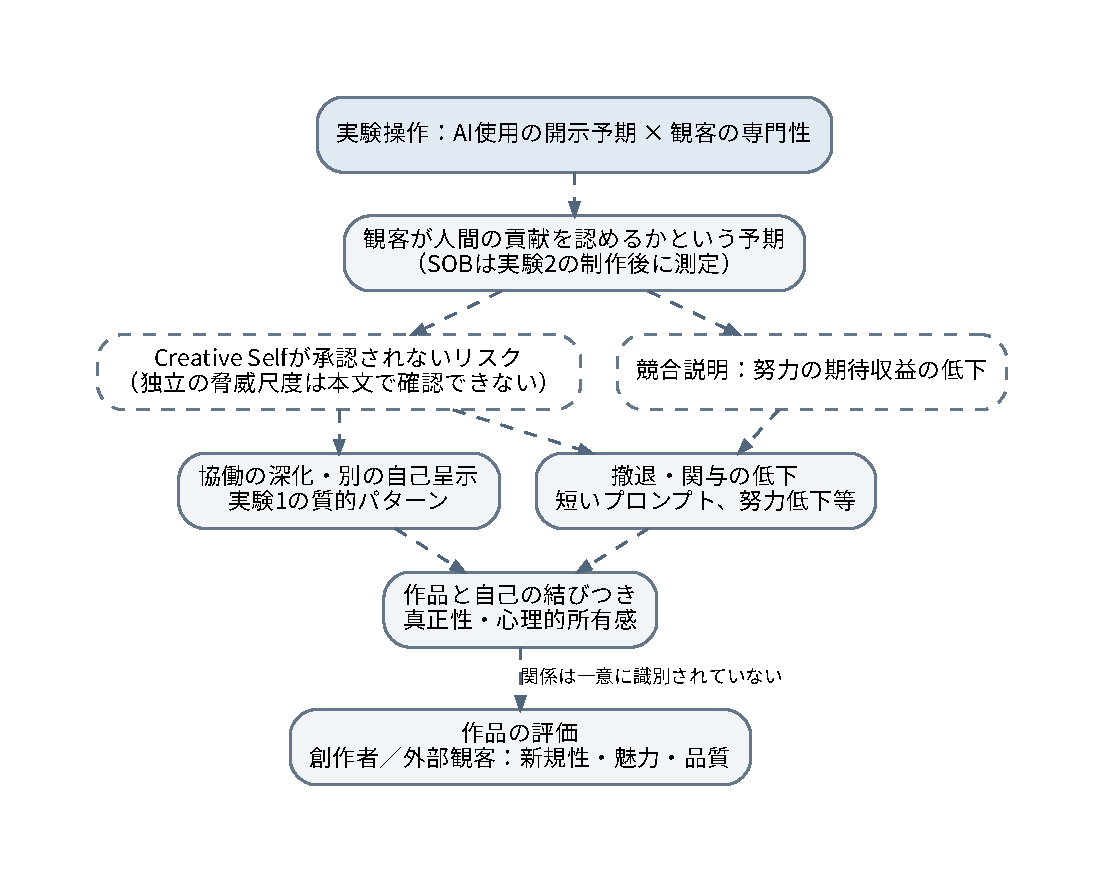
\includegraphics[width=0.88\textwidth,height=\textheight]{figures/process.pdf}
\caption{図2　間接開示効果の説明用概念パス図。破線＝仮説的・未識別の機構。各矢印は推定済み媒介効果ではない。}
\end{figure}

（1）協働の深化：AI利用を隠せないなら、AIを巧みに使う創作者としての自己を呈示する。（2）撤退：人間の貢献を承認してもらえないなら、作品を自分の自己表現として扱わず、AIに多くを委ねることで自己と作品の結びつきを弱める。実験1では両パターンが記録され、著者は後者が優勢と解釈した。撤退は自己防衛以外の理由でも説明可能である。

\section{9.
実験と測定の監査}\label{ux5b9fux9a13ux3068ux6e2cux5b9aux306eux76e3ux67fb}

\subsection{9.1
二つの実験の構造}\label{ux4e8cux3064ux306eux5b9fux9a13ux306eux69cbux9020}

Figure 2 (Jussupow p.~7)
は、創作者段階と評価者段階を分け、さらに二つの実験を区分する。実験1：27名のデザイン大学院生が「what
is
beauty?」について2作品を作成、54作品、279ページの制作記録、886分のインタビュー。制作段階は参加者内、評価段階は開示ラベルの参加者間比較。実験2：118名が
DALL-E 3 で「a portrait of a good
life」を1作品、15--30分で制作。2×2（開示予期／非開示予期 ×
一般観客／AI利用に熟知した観客）、各群30, 26, 31,
31人。1,095件のプロンプト。提出後に自己評価・自由記述・観客反応についての信念を測定。別の観客が成果物を評価する。

\subsection{9.2 Table
2（p.~14）の変数と役割}\label{table-2p.-14ux306eux5909ux6570ux3068ux5f79ux5272}

\begin{longtable}[]{@{}
  >{\raggedright\arraybackslash}p{(\columnwidth - 4\tabcolsep) * \real{0.3333}}
  >{\raggedright\arraybackslash}p{(\columnwidth - 4\tabcolsep) * \real{0.3333}}
  >{\raggedright\arraybackslash}p{(\columnwidth - 4\tabcolsep) * \real{0.3333}}@{}}
\toprule\noalign{}
\begin{minipage}[b]{\linewidth}\raggedright
変数群
\end{minipage} & \begin{minipage}[b]{\linewidth}\raggedright
測定内容
\end{minipage} & \begin{minipage}[b]{\linewidth}\raggedright
何を直接測らないか
\end{minipage} \\
\midrule\noalign{}
\endhead
\bottomrule\noalign{}
\endlastfoot
Prompt length / Number of prompts / Reported effort &
人間の関与に関連するログと自己申告 & 創造性・主体性の全体 \\
Creators' feelings / personality / True inspiration / Authentic work /
Honest work & 作成画像についての真正性関連の判断（5変数） &
創作者の恒常的なCPI・CSC \\
Psychological ownership & 作成画像と自己の心理的所有関係 &
法的所有権、自己全体 \\
Perceived novelty / appeal / quality & 作成画像についての自己評価 &
将来の遂行可能性（CSE） \\
Beliefs about audience responses (E3/E9) & 観客の反応に関する本人の予想
& 実際の観客反応、自己への脅威の強度 \\
\end{longtable}

本文 pp.~13--15：一般観客のもとで開示を予期すると、プロンプト長
−31.9\%、自己申告努力 −13.9\%、個性の反映 −20.4\%、着想
−11.1\%（p\textless.10）、真正性 −9.3\%、所有感
−25.2\%。観客が努力を認めるという予想 −18.4\%、誠実性の評価予想
−17.6\%（両方
p\textless.05）。これらは著者の相対的変化の報告であり、Creative Self
のスコアの変化ではない。専門家観客を予期すると、努力・個性・所有感・魅力・品質の交互作用は正で有意。専門家条件で有意な総効果は確認されなかったが、効果ゼロを証明するものではない。

\subsection{9.3
測定上の限界}\label{ux6e2cux5b9aux4e0aux306eux9650ux754c}

\begin{itemize}
\tightlist
\item
  Creative Self
  の独立した尺度や潜在変数モデルは最終版本文に確認できない。観客反応の予想、作品への自己投影、所有感、行動が同一因子である根拠もない。
\item
  SOB
  は制作後に測定されるため、制作前の承認予期が撤退を引き起こしたという時間的順序を直接観察していない。操作と行動の効果、機構に整合的な証拠は区別する。
\item
  作品の関与・評価が変化しても、自己の重要性、能力の自己信念、承認への懸念のどれが変化したかは確定できない。
\item
  p.~18 §6.4
  は努力への期待収益の低下等の競合機構を認める。匿名の画像制作・短時間の場面のため、他の媒体や持続的な評判に一般化する際に慎重さが必要。
\item
  付録 A1/E3/E9/D1
  が必要。今回も出版社PDFが取得できなかったため、Jussupowの逐語的項目文・回答尺度・尺度の出典・事前登録の変更は本文で確認できた範囲以外を確定しない。Valsesia等の原尺度が確認できたことと、Jussupowが何を採用したかは別問題である。
\end{itemize}

\section{10.
評価者比較の研究に向けた概念選択}\label{ux8a55ux4fa1ux8005ux6bd4ux8f03ux306eux7814ux7a76ux306bux5411ux3051ux305fux6982ux5ff5ux9078ux629e}

Jussupow
の操作は「生成AIを使った創作者がその使用を開示されることを予期するか」であり、「人間とAIのどちらに評価されるか」ではない。評価者がAIならば人間的な承認が得られないと感じる可能性、反対に人間よりも偏見なく評価されると期待する可能性があり、効果の方向は自動的に定まらない。

\begin{longtable}[]{@{}
  >{\raggedright\arraybackslash}p{(\columnwidth - 4\tabcolsep) * \real{0.3333}}
  >{\raggedright\arraybackslash}p{(\columnwidth - 4\tabcolsep) * \real{0.3333}}
  >{\raggedright\arraybackslash}p{(\columnwidth - 4\tabcolsep) * \real{0.3333}}@{}}
\toprule\noalign{}
\begin{minipage}[b]{\linewidth}\raggedright
研究の問い
\end{minipage} & \begin{minipage}[b]{\linewidth}\raggedright
測定候補
\end{minipage} & \begin{minipage}[b]{\linewidth}\raggedright
注意
\end{minipage} \\
\midrule\noalign{}
\endhead
\bottomrule\noalign{}
\endlastfoot
評価者に創造性が認められると思うか &
承認期待・人間の貢献の認識についての予期（制作前） &
高評価期待と自己承認期待を分ける \\
作品を通して自己を表現するか & 自己表現・真正性（制作後） &
結果物が自己を反映する判断 \\
創作への関与が変わるか & 行動ログ・努力・改良の質 &
長さ・時間だけでは創造的主体性を保証しない \\
成果物が創造的か & 独立した領域適合評価者による成果物評価 &
実験操作としての評価者と成果物測定者を区別 \\
能力への自信が変わるか & 課題特異的CSE &
これはKarwowski/Banduraの別理論を導入する場合のみ \\
\end{longtable}

一般的な説明例：陶芸作品の作成前、「審査員が自分の意図や工夫を理解すると思うか」を尋ね、作成後「自分の意図が作品に表れているか」「自分のものと感じるか」を尋ねる。これらは概念説明用の項目であり、妥当性が検証された尺度ではない。短期実験で
Creative Self
自体の変化を研究したいのであれば、自己のどの側面をどのように測るかを追加定義・検証する必要がある。

\section{11.
文献調査の優先順位}\label{ux6587ux732eux8abfux67fbux306eux512aux5148ux9806ux4f4d}

\textbf{まず読む（一次資料を所持）：} Jussupow §2.1, §2.4, §5, §6.4 →
Baumeister pp.~142--146 → Leary \& Kowalski pp.~34--36, 43 → Amabile
pp.~1000--1002 → Valsesia pp.~897--901, 907--908 → Zhang pp.~1103--1105,
1108--1109 → Louie pp.~6--7, 9--10 → Reif pp.~1--4。Karwowski
pp.~397--404 は比較・用語の境界づけに用いる。追加原著では、Goffman
(1956) pp.~7--8, 66--69, 156、Manning p.~680、Schultze \& Brooks
pp.~714, 722--725、Harvey \& Berry pp.~504--508, 516--517、Pierce
pp.~86, 92--93、Inzlicht pp.~337--338, 342--344 を優先する。特に
Schultze \& Brooks p.~725 はAI評価への理論的拡張に不可欠。

\textbf{次に取得する（優先）：} Amabile \& Pratt (2016)
の創造的過程、Amabile (1996)、Schlenker (1986)、および必要に応じて
Goffman (1959) の Jussupow
が引用した版（提供済みの1956年版と区別）。原典リンクと引用用途は別冊
Evidence Ledger
の文献表に整理した。さらにオンライン付録と、各尺度の直接の出典・項目対応を照合する。

この理論体系を採用する場合には、Karwowski
を無理に中心に置く必要はない。むしろ Creative Self-Beliefs と Creative
Self-Presentation
を区別して、検証したい心理過程に最も近い構成概念を選択することが重要である。

\section{12.
v4：追加原著による理論の深化と修正}\label{v4ux8ffdux52a0ux539fux8457ux306bux3088ux308bux7406ux8ad6ux306eux6df1ux5316ux3068ux4feeux6b63}

\subsection{12.1
Goffman：自己呈示は行為であり、自己の特性尺度ではない}\label{goffmanux81eaux5df1ux5448ux793aux306fux884cux70baux3067ux3042ux308aux81eaux5df1ux306eux7279ux6027ux5c3aux5ea6ux3067ux306fux306aux3044}

提供版の標題紙は1956年、University of Edinburgh, Social Sciences
Research Centre, Monograph No.~2 と明示する（PDF 3）。Jussupow
が引用する1959年Doubleday版とは区別する。Introduction pp.~7--8（PDF
17--18）は、自ら形成した印象を守る防衛的実践と、相手がその印象を守る保護的実践を区別し、performance
を他の参加者に影響する活動全体と定義する {[}G01--G02{]}。Chapter III
pp.~66--69（PDF 76--79）は、何が観客に見えるかを front/back region
の区別から説明する {[}G03--G04{]}。Chapter VII p.~156（PDF
166）は、役割への同一化が深いと、その役割の呈示の失敗が自己概念を損なう可能性を示す
{[}G05{]}。

例えば写真家が展覧会で作品を見せる行為は自己呈示である。編集前の失敗作を観客から隠すことは舞台裏の管理であり、写真家としての能力がないことを意味しない。観客から技量を否定されれば、写真家という役割への同一化が強いほど自己に関わる問題となりうる。しかし、Goffman
の議論はその影響の大きさや短期変化を定量化するものではない。Jussupow
の創造的自己への拡張は、創作物を呈示の媒体とする文脈固有の理論化である。

\subsection{12.2
Manning：承認の原文を厳密に読む}\label{manningux627fux8a8dux306eux539fux6587ux3092ux53b3ux5bc6ux306bux8aadux3080}

p.~680（PDF 4）で Manning は、performance
を観察可能な行動として、response
をその行動に続く相互作用として記述する。Jussupow p.~5 が引用する ``as
existing or having meaning'' の原文の対象は first
move（最初の行為）であって、直接には自己の存在ではない
{[}M01{]}。したがって「Manning
が自己の承認をその文で定義した」と記述するのは過剰である。Jussupow
は相互作用で行為が応答を受けるという命題を自己の社会的承認に拡張している。

同ページには応答が得られず、誤解され、無視される場合の疎外・困惑・撤退・防衛・再試行という複数の反応が列挙される
{[}M02{]}。p.~686（PDF
10）は自己そのものより呈示・相互作用を重視するという Manning
の解釈を示す
{[}M03{]}。例えば発表で質問を受けることは、必ずしも肯定的評価ではなくとも、その行為が意味あるものとして扱われたことを示しうる。承認と好意、賞賛、正の評価を同一視してはいけない。

\subsection{12.3 Schultze \&
Brooks：社会的存在とAI評価の理論的な断絶}\label{schultze-brooksux793eux4f1aux7684ux5b58ux5728ux3068aiux8a55ux4fa1ux306eux7406ux8ad6ux7684ux306aux65adux7d76}

原著は2018年オンライン公開、2019年巻号掲載（29, 707--737）。Second Life
の二つの相互作用を同一利用者の報告から質的に比較し、媒体の機能ではなく、人々が相互作用を通じて互いを心理的・情緒的に現実の存在として構成する過程を理論化した（p.~707,
p.~714）{[}S01--S02{]}。実験的に三段階の因果効果を推定した研究ではない。

\begin{longtable}[]{@{}
  >{\raggedright\arraybackslash}p{(\columnwidth - 4\tabcolsep) * \real{0.3333}}
  >{\raggedright\arraybackslash}p{(\columnwidth - 4\tabcolsep) * \real{0.3333}}
  >{\raggedright\arraybackslash}p{(\columnwidth - 4\tabcolsep) * \real{0.3333}}@{}}
\toprule\noalign{}
\begin{minipage}[b]{\linewidth}\raggedright
段階
\end{minipage} & \begin{minipage}[b]{\linewidth}\raggedright
原著 pp.~722--723（PDF 16--17）
\end{minipage} & \begin{minipage}[b]{\linewidth}\raggedright
説明例
\end{minipage} \\
\midrule\noalign{}
\endhead
\bottomrule\noalign{}
\endlastfoot
1 Copresence & 他者が存在し互いに観察可能と認識する &
オンライン会議に他者がいるとわかる \\
2 Focused interaction & 共通の活動に注意を割き適切に応答する &
一緒に曲を聴き、感想を交換する \\
3 Interlocking involvement obligation & 相互の関与と社会的自己を支え合う
& 相手の意図や感情を理解し、互いの自己呈示を認める \\
\end{longtable}

Table 1
とその説明（pp.~720--723）では、高い社会的存在が成立するためには、単に相手がいると感じるだけでなく、互いの社会的自己を支えることが必要と論じる
{[}S03--S04{]}。仮想環境の人間は実在の相手である。

\textbf{最重要の新知見：p.~725（PDF 19）。}
著者は自律AIとの会話への理論的拡張を明示的に検討する。第1・第2段階は成立しうるが、第3段階は成立しにくいと推論する。AIは人間から自己を承認されなければ困る存在ではなく、自己を守る動機に基づいて応答しているわけでもない
{[}S05{]}。さらにAIの承認が有効に機能しない可能性も示す
{[}S06{]}。プログラムされた応答と、人間の予測不能な反応が伴うリスクとの違いが理由である。ただし、これらはAI条件を実験して得られた結論ではなく理論的な議論である。

したがって、AIを評価者とする今回の研究にこの文献を用いる価値は極めて高い。Jussupow
の人間観客をAIに置き換えても同じ社会的承認が成立すると仮定するのではなく、評価主体によって承認の期待・価値・リスクが異なるかを検証する理論的根拠になる。方向は一意ではない。AIが自分の表現を理解してくれないため努力を減らす可能性も、人間からの否定的評価を恐れなくてよいため自由に表現する可能性も考えられる（本資料の仮説）。

\begin{figure}
\centering
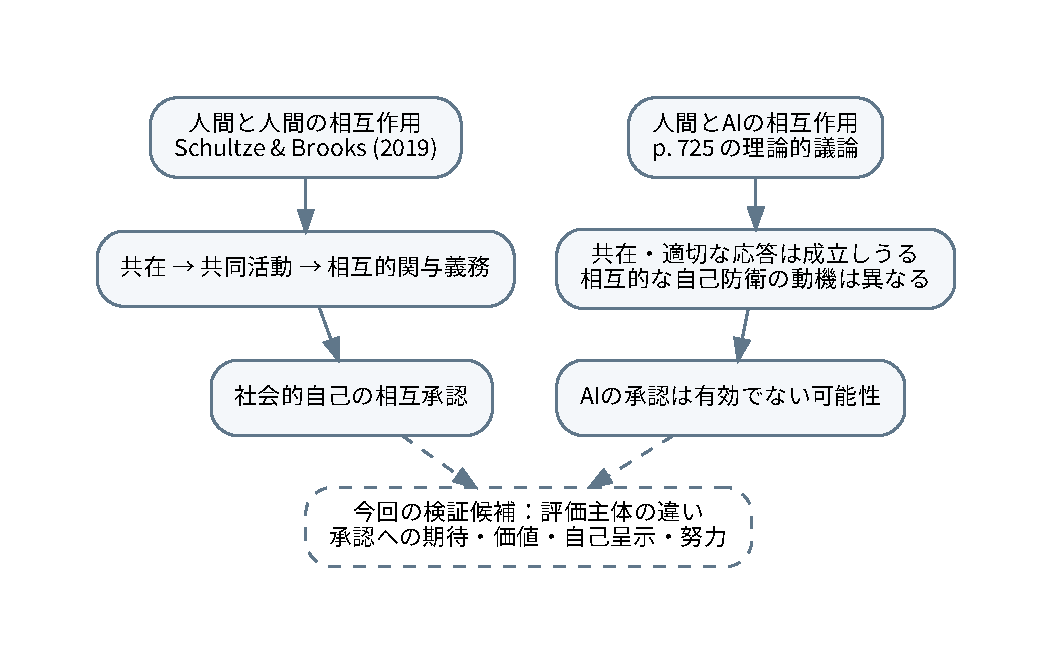
\includegraphics[width=0.96\textwidth,height=\textheight]{figures/validation_boundary.pdf}
\caption{図3　人間評価とAI評価を比較するための理論上の境界。実線は文献の議論、破線は今回の研究における検証候補。}
\end{figure}

\subsection{12.4 Harvey \&
Berry：新規性と有用性、創作の三形態}\label{harvey-berryux65b0ux898fux6027ux3068ux6709ux7528ux6027ux5275ux4f5cux306eux4e09ux5f62ux614b}

この理論論文は新規性と有用性が創造性の共通要素である一方、その定義・関係・生成過程は一様でないことから、三つの形態を導出する（pp.~504--505,
Table 1 p.~508）{[}H01--H02{]}。

\begin{longtable}[]{@{}
  >{\raggedright\arraybackslash}p{(\columnwidth - 4\tabcolsep) * \real{0.3333}}
  >{\raggedright\arraybackslash}p{(\columnwidth - 4\tabcolsep) * \real{0.3333}}
  >{\raggedright\arraybackslash}p{(\columnwidth - 4\tabcolsep) * \real{0.3333}}@{}}
\toprule\noalign{}
\begin{minipage}[b]{\linewidth}\raggedright
形態
\end{minipage} & \begin{minipage}[b]{\linewidth}\raggedright
新規性と有用性の関係
\end{minipage} & \begin{minipage}[b]{\linewidth}\raggedright
一般例
\end{minipage} \\
\midrule\noalign{}
\endhead
\bottomrule\noalign{}
\endlastfoot
Maximization & 新規案を広く生成し、後に有用な案を選択する &
小説の題材を自由に考える \\
Balance & 両者を比較・調整しながら案を具体化する &
出版社への企画提案を独自性と市場適合性の両面から修正する \\
Integration & 具体的な制作の中で新規性と有用性を同時に形成する &
執筆中に表現・登場人物・物語構造を一体として工夫する \\
\end{longtable}

pp.~516--517（PDF
13--14）の執筆例は、書くという行為自体が創造的過程となりうること、目的との適合性が有用性を意味しうることを示す
{[}H03{]}。したがって目的を持つ文章課題でも創造性を発揮する余地はある。ただし、志望動機という特定課題が妥当な創造性課題であることを直接検証した研究ではない。課題に複数の妥当な表現や構成の可能性があり、単なる定型文の再現ではないことを別途示す必要がある。

Jussupow p.~3
はアイデアの生成と成果物への実現を区別するためこの文献を使う。Creative
Agency の直接定義は Jussupow 自身による概念化であり、Harvey \& Berry
の三形態を Creative Self の下位因子にする根拠はない。

\subsection{12.5
Pierce：心理的所有感を自己との関係として理解する}\label{pierceux5fc3ux7406ux7684ux6240ux6709ux611fux3092ux81eaux5df1ux3068ux306eux95a2ux4fc2ux3068ux3057ux3066ux7406ux89e3ux3059ux308b}

Psychological Ownership
は所有対象を自分のものと感じる認知的・感情的状態である（p.~86）{[}P01{]}。著者はその動機として
efficacy/effectance、self-identity、居場所の三つを論じる（p.~84）{[}P02{]}。さらに所有感が形成される経路は対象への統制、対象を深く知ること、自己を投入することの三つである（p.~92）{[}P03{]}。この三経路は理論的な説明であって、心理的所有感尺度の三因子ではない。

たとえば自分で木材を選び、加工し、設計を修正した家具は、自分のものと感じやすいかもしれない。誰かが作った家具でも長期間使用して深く知れば所有感を持つことがある。一方、所有感は作者としての社会的承認とも、創造性が自己にとって重要かとも異なる。Jussupow
の創作への関与・作品との結びつきを説明する補助理論として有用だが、Creative
Self 自体の直接尺度を提供するわけではない。

\subsection{12.6
Inzlicht：努力と創造的主体性を混同しない}\label{inzlichtux52aaux529bux3068ux5275ux9020ux7684ux4e3bux4f53ux6027ux3092ux6df7ux540cux3057ux306aux3044}

努力は目標に向けた精神的・身体的活動の主観的な強化である（p.~338）{[}E01{]}。能力、課題難易度、動機づけとは区別される。レビューの中核は努力がコストでありながら、成果の価値や努力それ自体に正の価値を付加しうるという点である（pp.~337,
342）{[}E02--E03{]}。pp.~344--345
の議論は努力の価値を成果中心と努力自体中心のモデルで整理する。

例えば自作の家具に高い価値を感じる人は、他者から評価されなくても作る過程に価値を見いだしうる。逆に努力が報われないと考え、効率的な方法を選ぶ人もいる。Jussupow
p.~18
は努力への期待される見返りに基づく撤退を自己防衛とは別の説明として挙げている。Inzlicht
の原著は AI
評価や自己防衛のメカニズムを直接比較したものではない。実験で努力の低下を観察しても、その原因を自己防衛に一意に帰属できない。

\section{13. 定義から測定への対応：v4
の整理}\label{ux5b9aux7fa9ux304bux3089ux6e2cux5b9aux3078ux306eux5bfeux5fdcv4-ux306eux6574ux7406}

\begin{longtable}[]{@{}
  >{\raggedright\arraybackslash}p{(\columnwidth - 4\tabcolsep) * \real{0.3333}}
  >{\raggedright\arraybackslash}p{(\columnwidth - 4\tabcolsep) * \real{0.3333}}
  >{\raggedright\arraybackslash}p{(\columnwidth - 4\tabcolsep) * \real{0.3333}}@{}}
\toprule\noalign{}
\begin{minipage}[b]{\linewidth}\raggedright
理論上の役割
\end{minipage} & \begin{minipage}[b]{\linewidth}\raggedright
概念
\end{minipage} & \begin{minipage}[b]{\linewidth}\raggedright
何が観察可能か
\end{minipage} \\
\midrule\noalign{}
\endhead
\bottomrule\noalign{}
\endlastfoot
定義の対象 & Creative Self & Jussupow
の定義。直接的な検証済み総合尺度は確認できない \\
相互作用の機構 & Self-presentation / Social validation &
自己を表現する意図、認められるという期待、認められたと感じる程度（別々の変数） \\
制作過程 & Creative Agency / Effort &
選択、編集、修正等の記録と努力の自己報告。努力単独は主体性の完全な指標ではない \\
作品と自己 & Authenticity / Ownership &
自己の意図・個性を表現する程度と自分のものと感じる程度 \\
成果 & Creativity / Quality &
独創性・課題適合性、外部評価、自己評価。好意とは区別 \\
境界条件 & Social presence / 承認の価値 & AI
と人間の承認が同等か、評価者をどの程度意味ある他者と感じるか（追加検証候補） \\
\end{longtable}

\textbf{実験設計への結論：} Jussupow と整合する研究にするには、Creative
Self
が低下したかという曖昧な問いより、評価主体の通知が自己呈示、予期される社会的承認、創造的主体性、作品との結びつきにどう影響するかを明示する。Karwowski/SSCS
は独立した自己信念やアイデンティティを測定したい場合の選択肢であって必須ではない。Goffman
と Schultze \& Brooks
の議論を用いる場合でも、AIによる社会的承認が同様に機能するかは仮説として扱う。

残る未確認事項は Jussupow オンライン付録、Amabile \& Pratt
(2016)、Amabile (1996)、Schlenker (1986)
等である。既存尺度を実験に適応する際は原項目と新項目、回答尺度、測定時点、妥当性の検証を別途記録する。

\end{document}
